\chapter{Background}
\label{chap:background}
\lhead{\emph{Background}}
The key question to answer in this chapter is: "What has been done/is being done". 

This chapter comprises around 4000 words and should put your project into context within Computer Science. Your focus here should be on the final section "Current State of the Art". This should be at least 2500 of the 4000 words of this section.

\section{Thematic Area within Computer Science}
The Core topic of this project is safely and dynamically encrypting messages between two parties. The communication will rely on multiple functioning NodeJs servers for transfer of encrypted messages. 

The core areas under which my project falls under is cryptography, security for encrypting and securing information. Machine learning will be used for establishing methods of secure information exchange. And finally networking due to the setup required of communicating between different servers and sending encrypted information.

Encryption \cite{encryptionDefinition} is when the plaintext of any form of data that can be easily read is converted to an unreadable encoded version. In order to retrieve the original data for viewing or processing it must be decoded using a specific algorithm and more than likely some sort of key, usually a lengthy password. Encryption may be used for encrypting files and operating systems on a user's hard drive. In today's world encryption is used religiously for data transferred between networks. Sensitive information like user's credentials are constantly being sent from the browser to the server when logging into websites for personalised content. The same is true for for even more high risk information like banking details, scans of identification documents and even keys. Websites that wish to be secure are now using HTTPS instead of HTTP. The Number of websites using HTTPS is constantly increasing see figure \ref{fig:httpsRise}

\begin{figure}[ht]
  \centering
      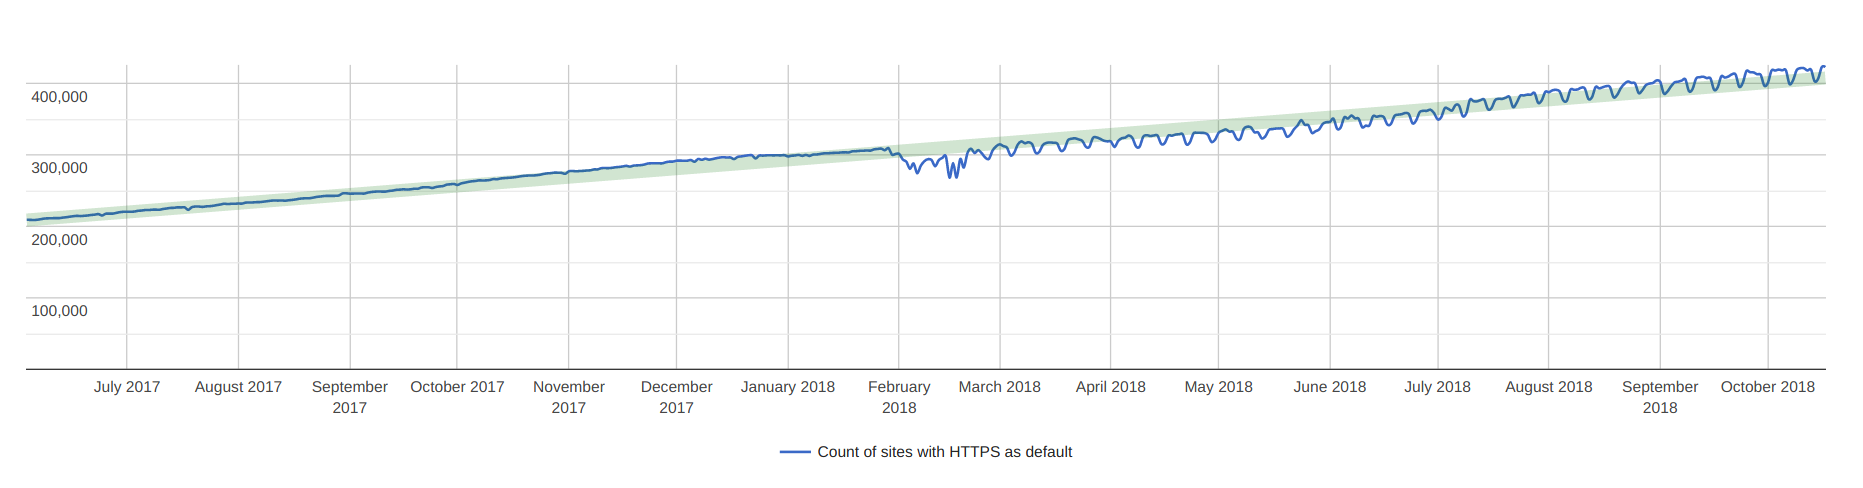
\includegraphics[width=0.9\textwidth]{Figures/httpsRise.png}
  \caption[A graph of HTTPS usage increase]{A graph of HTTPS usage increase\cite{https}}
  \label{fig:httpsRise}
\end{figure}

HTTP is not secure because information transmitted is in plaintext by default and extra steps are needed to encrypt the data. Because the author of the server can choose how the data is encrypted, it can lead to the theft of data as the implementation may not be correct or a weak algorithm is used.
On the other hand if a website uses HTTPS which is a common defined standard there will be minimal data theft see figure \ref{fig:https1}. HTTPS uses SSL or TLS which are protocols that use asymmetric keys (will be discussed later). SSL is generally used more often as it requires the server to acquire an SSL certificate from a trusted third party.

\begin{figure}[ht]
  \centering
      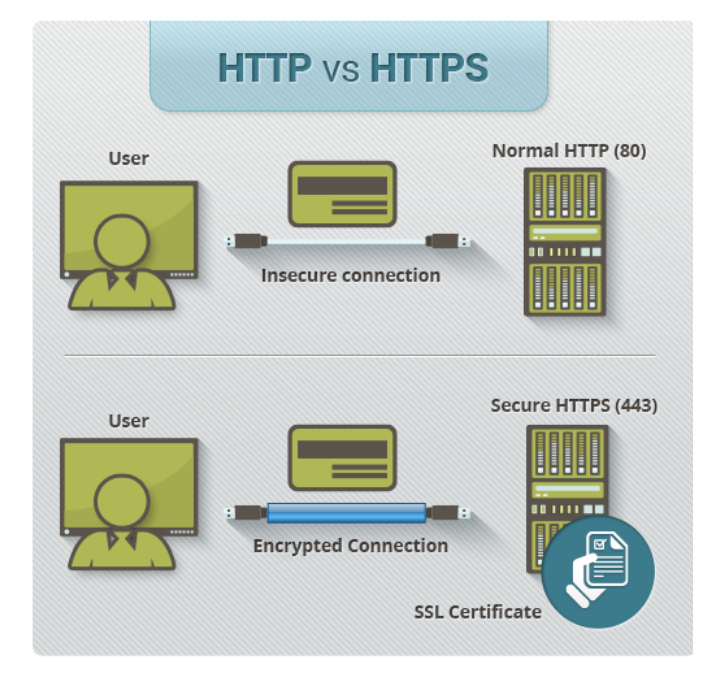
\includegraphics[width=0.6\textwidth]{Figures/httpsVsHttp.png}
  \caption[HTTP vs HTTPS]{HTTP vs HTTPS\cite{https1}}
  \label{fig:https1}
\end{figure}



Traditionally there are two encryption types.
\begin{enumerate}
    \item Symmetric
    \item Asymmetric
\end{enumerate}

Symmetric encryption uses the same key to encrypt and decrypt information. This type of encryption is usually used to encrypt information provided by a human generated key. It is not safe to send this key over a network as it can be stolen or the destination being sent to can be spoofed. There are multiple implementations of symmetric ciphers, the most common being AES, Twofish and Serpent. To increase your security at the cost of encryption and decryption time you can chain multiple ciphers together AES(Twofish(Key)).

Asymmetric or commonly known as public key encryption methods are commonly used for sharing data between between computers on different networks. This is because a set of keys are generated one being private and the other public. The private key is never shared and remains on the host that generated it. The public key on the other hand can be shared with the party you want to communicate securely with. The public key is used to encrypt the data that is about to be sent back. This data can only be decrypted using the private key. Therefore you can share your public key with anyone and they wont be able to decrypt messages sent from another host who used the same public key. The most common algorithm is RSA. Certain protocols also use public key algorithms like SSH for secure remote connections to foreign hosts. And GPG for verification of packages on Linux systems and an alternative over https for Github.

Protocols like SSH create a set of keys during the start of the session and those keys remain constant therefore if the private key was leaked the whole conversation could be decrypted if the packets have been captured and stored.  

Encryption in its general form is simply a mathematical algorithm that takes plaintext and combines it with some sort of key over a number of iterations eventually producing the ciphertext. This might entice some people to try and break those ciphers and recover the original plain text. Quite a number of attacks do exist.
Private keys are sometimes stored on the disk or in temporary files that are saved by programs during their execution, until reboot or they are cleared after a number of days. The attacker may be able to access the server physically or remotely using an unrelated exploit and copy the key.

Social engineering is an attack where a human pretends to be of an authority figure and convinces an unaware human to give up the key. This can be done by an attacker pretending to be an executive engineer in a company and convince the victim indirectly or directly to give up the keys by running obfuscated commands in the terminal which then send over the key to the attackers server.

If the key used is created by a human and not some sort of machine generator there are a few number attacks that can be performed that would not be feasible or possible if the key was generated or quite long. These attacks include brute force which creates keys in usually ascending order or based on some algorithm to increase the chance of success. Brute force will eventually try every key possible however even a small sized key of 12 characters containing numbers, symbols, upper and lover case numbers it would take around 200 years \cite{brute}. 
Dictionary attacks can be used if the key is part of a large dictionary of human created passwords. 

Attacks on proper keys that are generated by machines are more sophisticated and rely on cracking the algorithm or device used for encryption more so then the key.
Linear cryptanalysis \cite{cipher-attacks} is a plaintext attack which means that the attack can use any plain text they want and receive the ciphertext for it after putting it through a system. This attack uses linear approximations to describe the behaviour of the block cipher. After large number of pairs of plaintext and cipher text there is a possibility to learn something about the key.

Algebraic attacks \cite{cipher-attacks} can be used if the ciphers exhibit a high probability of a mathematical structure. 

Reverse Engineering \cite{cipher-attacks} can be used to either examine the source code of the algorithm or disassemble the binary which uses the algorithm to look as the assembly code of the algorithm.
Machine key generators usually use some form of a random number generator which are algorithms that usually take in a seed hopefully something that isn't the current time but that has been known to be used and return a key. Attacks can be made on this number generator if the seed is something predictable or the generator generates predictable numbers. 

If the device on which the algorithm is performing on is an embedded device you can perform side channel attacks \cite{cipher-attacks} where you measure the spikes and frequency of the power consumption when the encryption is taking place. 

%
%
% End of encription 
%
%

Machine learning is a category of algorithms that allow systems to automatically learn and improve from experience without being explicitly programmed \cite{machineLearning}. Basically this means that the algorithm can update when input is received this in turn updates the the output even if the same inputs are used later on.
Typically machine learning software processes large amounts of data and looks for patterns constantly updating either variables or adding logic branches. Recommendation engines use machine learning to personalise the logged in users feed. So if user one looked at product X and user 2 bought product X and also bought product Y then user one will most likely see product Y as a recommendation. There are three types of recommendation systems. Collaborative Filtering \cite{recommendation} where similarities between customers is taken into account.
Content Based Filtering \cite{recommendation} is when the liked and purchased items are taken into account. See figure \ref{fig:recommendation} for illustration.
Finally there is Hybrid Recommendation Systems which is a mix between the previous two and is typically the one used in industry.

\begin{figure}[ht]
  \centering
      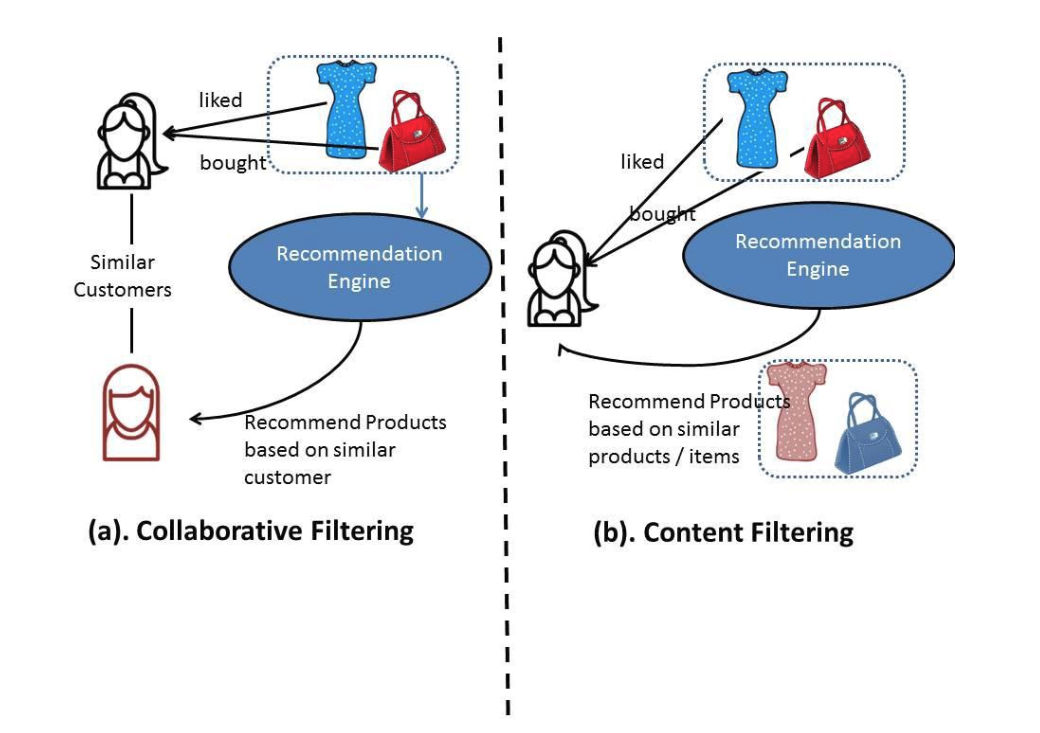
\includegraphics[width=0.9\textwidth]{Figures/recommendationEngine.png}
  \caption[An example of recommendation engine]{An example of recommendation engine\cite{recommendation}}
  \label{fig:recommendation}
\end{figure}

The most common machine learning algorithms are often classified as supervised learning and unsupervised learning.
Supervised learning \cite{supervised} relies on a set of training data which is constructed of various inputs and and correct outputs corresponding to those inputs usually labels. The training data is usually left unchanged and when the test data or data taken from the current user is used as input the algorithm attempts to correctly classify the data based on the training data. The disadvantage of supervised learning is if the incoming data is radically different from the test data the probability of classifying the data into the correct label will be similar and sometimes even lower than classifying into the incorrect label. However because the training data exists it can be quite quicker to setup a supervised learning system then an unsupervised.

Unsupervised learning \cite{unsupervised} uses data that is neither classified or labelled. This allows the algorithm to draw its own conclusions about the data as well as discover hidden structures. If some of the data is similar in any way to another piece of data the algorithm tends to group those pieces of data together. Unsupervised learning is generally more complex and can be more accurate since the algorithm might find subtle discrepancies that might be impossible to notice for a human. This however can lead to unpredictable behaviour where there is expected to be two classifications but instead the data is classified into a lot more than two classifications. Unsupervised learning algorithms typically require more training data than supervised in order to detect similarities and come up with labels.

There are also algorithms that use techniques found in both supervised and unsupervised machine learning these are called Semi-supervised \cite{machineLearning0} machine learning these use a much larger amount of unlabelled training data than labelled. These types of algorithms usually tend to be more accurate than supervised and unsupervised alone.

Another interesting suite of machine learning algorithms is classified into Reinforcement Learning \cite{reinforcementLearning}. These algorithms interact with the environment and received rewards or penalties based on the actions carried out within the environment. If the action carried out receives a reward it is likely that the same action will be repeated again. 

Achieving synchronisation \cite{sync} is an important part of this project. 
Synchronisation is the process of making two or more data storage devices or programs (in the same or different computers) having exactly the same information at a given time.
Synchronisation is common in multi-threaded software where any number of threads can manipulate the same set of data or even wait for a certain thread to finish execution. For example you wouldn't want your parent thread to finish before the child threads as this can lead to data loss and resources being hogged by a zombie thread. Pthread \cite{pthread} is a great API that can be used for handling threads and shared data between those threads. 









%
%
% Stick these somehwere maybe
%
%
Machine learning has been known to be used for secure communications although it is not clear if it is used in servers with valuable data. Google's AI successfully created secure algorithms \cite{GoogleAi1} that use inhuman cryptographic schemes making them harder to crack. This technique is called GAN Cryptography \cite{GoogleAi2} for which a research paper can be found.

Currently dynamic encryption is exercised in voip phone calls by a company known as Dencrypt \cite{dencrypt} according to the explanation of their proprietary algorithm they use a wrapper on top of AES-256 which is a chosen algorithm that is discarded when the data transfer is finished.


This project will be compatible with NodeJs because it is one of the fastest growing server platform \cite{NodeJs} that can be easily set up and supports a large amount of modules.




Position your topic within Computer Science. This activity will aid you in your literature review also. We zoom out to see three levels:

% notice the enumerate structure to create itemized lists
\begin{enumerate}
    \item What is the core topic your project is about? e.g., Mobile app for online voting.
    \item What core area(s) does the project fall under? e.g., Mobile applications, Social Networking, Service Providers. 
    \item What main area(s) of Computer Science does the project fall under? e.g. Software Development, Cloud Computing.
\end{enumerate}

The ACM Computing Classification System (http://www.acm.org/about/class) will aid you in this, use the 2012 categories. Make sure to use figures and illustrations were appropriate. LaTeX will take care of the formatting of these. Do not try to get fancy here, you should concentrate on the content and not the formatting, this is why we are specifying LaTeX.

% Again take note of the structure, simply copy and paste this for future single figures
\begin{figure}[ht]
  \centering
      
\includegraphics[width=0.7\textwidth]{successkid.jpg}
  \caption[A picture of the success kid!]{A picture of the success kid!\cite{Reference1}}
  \label{fig:successkid}
\end{figure}

You can specify the width and label for a figure which allows you to reference the figure and you can attribute a source in the figure caption as is done for figure \ref{fig:successkid}. Make sure you reference all external figures (i.e. figures you did not create yourself). Also use references for all figures e.g. use "... in figure \ref{fig:successkid} ..." NOT "... in the figure above ...".

%\section{Project Scope}
%Project specifics: Background minimum knowledge.

%Imagine you wanted to explain the specifics of your project to a person that knows nothing of Computer Science. You cannot talk about everything (as the idea is not to write a 500+ page report). Remember the reader at this stage can only be assumed to know what you have covered, so identify what are the minimum concepts belonging to the main areas (listed as 3 in the section before) and the core areas (listed as 2 in the section before) that you would need to explain so that the reader is able to understand the specifics of your project and indeed the following section. For example the minimum amount of knowledge about software development, cloud computing, mobile applications, social networking and service providers that are required so as to understand the specifics of a project about a mobile app for an on-line voting system. Here we are making the same trip we did before, but now in the opposite direction. Start zooming in from 3, then to 2 and finally to reach your project 1. Once the reader is finished this section they should be able to understand the proceeding sections (and have context for it within the project).

\section{A Review of -INSERT THEMATIC AREA-}
The focus of this section is at the heart of the project research phase. You must identify the main sources of information you should be aware of within your chosen area and pay regular attention to so as to strengthen your knowledge in the core topic you are working at. So here you should develop an knowledge of not only your core topic but also about the area of computer science the topic falls under. More specifically you should research the following:
\begin{itemize}
    \item The top 5 International Conferences and Journals most related to your topic. This is crucial, as it represents the main source for keeping you aware of what the state-of-the-art in your topic is.
    \begin{itemize}
        \item In particular it will make you aware of what other projects related to yours have been already done (so that you can compare/position your project w.r.t. these).
        \item What new techniques are being developed, so that you can apply them in your work. e.g. new frameworks for data visualization
    \end{itemize}
    \item The top 3 most recent books/texts related to your topic. There are many free resources from which you may download a relevant text on the topic of your project. Try to either download or borrow 3 recent (no older than 10 years) texts relating to the topic your project is on which you will use throughout the project as reference material and to aid in tackling a number of the technical problems you may encounter. Any PhD/MSc thesis that have published in the last 5 years relating to the topic are also invaluable resources as they will contain a state of the art and references in your project topic. Approach these only after reading/viewing the wikis/Youtube videos you find as a certain level of knowledge will be assumed about the topic.
    \item The top 5 companies/organizations potentially interested in the product you are developing. Finally, this is also crucial, as it forces you extend to purely programmer view of the project to a wider view considering the market, potential stakeholders and niches where your product can become useful. Moreover, Computer Science is a huge topic with loads of different works and roles. If you pick a project in the area you feel passionate about, and you identify what the market in this area is about, then you can drive your future professional career (from the very beginning) towards the path that makes you happier. I know that this does sound as a very technical reason, but I suppose we all agree is probably the most important of all reasons for choosing a particular project focus. 
    \item The top 5 wiki/forums/blogs/Youtube channels most related to your topic. This is crucial to you as well, as it represents a more accessible, personal and less informal way of communication with people working/interested on the same topic as you are. This communication is extremely helpful for improving your skills, solving potential doubts and increase the interest/relevance of the topic/area itself.
\end{itemize}

You should begin your journey of discovery in reverse order to the listing above (which is given in order of academic importance/significance). So when you are researching your topic first look up some TedX talks or youtube tutorials, then research what companies are doing in the area, then get a handful of very good texts on the core topics of your area (anything older than 5 years usually is not helpful here) and finally start reading conference or journal papers (again newer is better here). In particular during this section you may need to use tables to list resources. These are also automatically formatted in latex thus allowing you to concentrate on content. for example table \ref{tab:Mylar}.

\begin{table}[ht]
	\centering
		\begin{tabular}{ c  c  }
		\hline
		\hline
		Parameter & PET \\
		\hline
		Youngs Modulus & 2800-3100MPa \\
		Tensile Strength & 55-75MPa \\
		Glass Temperature & 75$^\circ$C \\
		Density & 1400kg/m$^3$ \\
		Thermal Conductivity & 0.15-0.24Wm$^{-1}$K$^{-1}$ \\
		Linear Expansion Coefficient & $7\times10^-5$ \\
		Relative Dielectric Constant @ 1MHz & 3\\
		Dielectric Breakdown Strength & 17kVmm$^{-1}$\\
		\end{tabular}
	\caption{PET Physical Properties}
	\label{tab:Mylar}
\end{table}

What has been done before in your community w.r.t. your topic? Once you have gotten an understanding of the topic and technologies and have identified the top 5 formal conferences/journals, wiki/forums/blogs/Youtube channels and companies/organizations the next step is to research in depth on them! And here in depth means in depth. Make sure you cite\cite{Reference1} a number of papers \cite{Reference3}, luckily Latex will take care of the ordering of the citations \cite{Reference2} for you.

The aim here is that you find the trends in your topic (3), and more in general in the area in which your topic resides (2) your project falls under and from these trends you develop your initial project question further and begin to get insights into how others have solved/approached similar problems. Think of this section as colouring in your initial idea. Before you approach this section you should read at least 4/5 good literature reviews (a selection of last years projects will be posted on blackboard to aid you but you should find other sources also).

In particular in this section, you must find and analyze at least 5 (ideally around 10) works belonging to, or at least related to, your work. You must describe these works and position your project w.r.t. them (i.e., clearly identify the similarities and differences between your project and each of these works). Also remember if you find that you are detailing topics that you have not introduced already here you need to add something to the earlier Scope section.